
%% bare_conf.tex
%% V1.4b
%% 2015/08/26
%% by Michael Shell
%% See:
%% http://www.michaelshell.org/
%% for current contact information.
%%
%% This is a skeleton file demonstrating the use of IEEEtran.cls
%% (requires IEEEtran.cls version 1.8b or later) with an IEEE
%% conference paper.
%%
%% Support sites:
%% http://www.michaelshell.org/tex/ieeetran/
%% http://www.ctan.org/pkg/ieeetran
%% and
%% http://www.ieee.org/

%%*************************************************************************
%% Legal Notice:
%% This code is offered as-is without any warranty either expressed or
%% implied; without even the implied warranty of MERCHANTABILITY or
%% FITNESS FOR A PARTICULAR PURPOSE! 
%% User assumes all risk.
%% In no event shall the IEEE or any contributor to this code be liable for
%% any damages or losses, including, but not limited to, incidental,
%% consequential, or any other damages, resulting from the use or misuse
%% of any information contained here.
%%
%% All comments are the opinions of their respective authors and are not
%% necessarily endorsed by the IEEE.
%%
%% This work is distributed under the LaTeX Project Public License (LPPL)
%% ( http://www.latex-project.org/ ) version 1.3, and may be freely used,
%% distributed and modified. A copy of the LPPL, version 1.3, is included
%% in the base LaTeX documentation of all distributions of LaTeX released
%% 2003/12/01 or later.
%% Retain all contribution notices and credits.
%% ** Modified files should be clearly indicated as such, including  **
%% ** renaming them and changing author support contact information. **
%%*************************************************************************


% *** Authors should verify (and, if needed, correct) their LaTeX system  ***
% *** with the testflow diagnostic prior to trusting their LaTeX platform ***
% *** with production work. The IEEE's font choices and paper sizes can   ***
% *** trigger bugs that do not appear when using other class files.       ***                          ***
% The testflow support page is at:
% http://www.michaelshell.org/tex/testflow/



\documentclass[conference]{IEEEtran}
% Some Computer Society conferences also require the compsoc mode option,
% but others use the standard conference format.
%
% If IEEEtran.cls has not been installed into the LaTeX system files,
% manually specify the path to it like:
% \documentclass[conference]{../sty/IEEEtran}





% Some very useful LaTeX packages include:
% (uncomment the ones you want to load)


% *** MISC UTILITY PACKAGES ***
%
%\usepackage{ifpdf}
% Heiko Oberdiek's ifpdf.sty is very useful if you need conditional
% compilation based on whether the output is pdf or dvi.
% usage:
% \ifpdf
%   % pdf code
% \else
%   % dvi code
% \fi
% The latest version of ifpdf.sty can be obtained from:
% http://www.ctan.org/pkg/ifpdf
% Also, note that IEEEtran.cls V1.7 and later provides a builtin
% \ifCLASSINFOpdf conditional that works the same way.
% When switching from latex to pdflatex and vice-versa, the compiler may
% have to be run twice to clear warning/error messages.






% *** CITATION PACKAGES ***
%
%\usepackage{cite}
% cite.sty was written by Donald Arseneau
% V1.6 and later of IEEEtran pre-defines the format of the cite.sty package
% \cite{} output to follow that of the IEEE. Loading the cite package will
% result in citation numbers being automatically sorted and properly
% "compressed/ranged". e.g., [1], [9], [2], [7], [5], [6] without using
% cite.sty will become [1], [2], [5]--[7], [9] using cite.sty. cite.sty's
% \cite will automatically add leading space, if needed. Use cite.sty's
% noadjust option (cite.sty V3.8 and later) if you want to turn this off
% such as if a citation ever needs to be enclosed in parenthesis.
% cite.sty is already installed on most LaTeX systems. Be sure and use
% version 5.0 (2009-03-20) and later if using hyperref.sty.
% The latest version can be obtained at:
% http://www.ctan.org/pkg/cite
% The documentation is contained in the cite.sty file itself.






% *** GRAPHICS RELATED PACKAGES ***
%
\ifCLASSINFOpdf
  % \usepackage[pdftex]{graphicx}
  % declare the path(s) where your graphic files are
  % \graphicspath{{../pdf/}{../jpeg/}}
  % and their extensions so you won't have to specify these with
  % every instance of \includegraphics
  % \DeclareGraphicsExtensions{.pdf,.jpeg,.png}
\else
  % or other class option (dvipsone, dvipdf, if not using dvips). graphicx
  % will default to the driver specified in the system graphics.cfg if no
  % driver is specified.
  % \usepackage[dvips]{graphicx}
  % declare the path(s) where your graphic files are
  % \graphicspath{{../eps/}}
  % and their extensions so you won't have to specify these with
  % every instance of \includegraphics
  % \DeclareGraphicsExtensions{.eps}
\fi
% graphicx was written by David Carlisle and Sebastian Rahtz. It is
% required if you want graphics, photos, etc. graphicx.sty is already
% installed on most LaTeX systems. The latest version and documentation
% can be obtained at: 
% http://www.ctan.org/pkg/graphicx
% Another good source of documentation is "Using Imported Graphics in
% LaTeX2e" by Keith Reckdahl which can be found at:
% http://www.ctan.org/pkg/epslatex
%
% latex, and pdflatex in dvi mode, support graphics in encapsulated
% postscript (.eps) format. pdflatex in pdf mode supports graphics
% in .pdf, .jpeg, .png and .mps (metapost) formats. Users should ensure
% that all non-photo figures use a vector format (.eps, .pdf, .mps) and
% not a bitmapped formats (.jpeg, .png). The IEEE frowns on bitmapped formats
% which can result in "jaggedy"/blurry rendering of lines and letters as
% well as large increases in file sizes.
%
% You can find documentation about the pdfTeX application at:
% http://www.tug.org/applications/pdftex





% *** MATH PACKAGES ***
%
%\usepackage{amsmath}
% A popular package from the American Mathematical Society that provides
% many useful and powerful commands for dealing with mathematics.
%
% Note that the amsmath package sets \interdisplaylinepenalty to 10000
% thus preventing page breaks from occurring within multiline equations. Use:
%\interdisplaylinepenalty=2500
% after loading amsmath to restore such page breaks as IEEEtran.cls normally
% does. amsmath.sty is already installed on most LaTeX systems. The latest
% version and documentation can be obtained at:
% http://www.ctan.org/pkg/amsmath





% *** SPECIALIZED LIST PACKAGES ***
%
%\usepackage{algorithmic}
% algorithmic.sty was written by Peter Williams and Rogerio Brito.
% This package provides an algorithmic environment fo describing algorithms.
% You can use the algorithmic environment in-text or within a figure
% environment to provide for a floating algorithm. Do NOT use the algorithm
% floating environment provided by algorithm.sty (by the same authors) or
% algorithm2e.sty (by Christophe Fiorio) as the IEEE does not use dedicated
% algorithm float types and packages that provide these will not provide
% correct IEEE style captions. The latest version and documentation of
% algorithmic.sty can be obtained at:
% http://www.ctan.org/pkg/algorithms
% Also of interest may be the (relatively newer and more customizable)
% algorithmicx.sty package by Szasz Janos:
% http://www.ctan.org/pkg/algorithmicx




% *** ALIGNMENT PACKAGES ***
%
%\usepackage{array}
% Frank Mittelbach's and David Carlisle's array.sty patches and improves
% the standard LaTeX2e array and tabular environments to provide better
% appearance and additional user controls. As the default LaTeX2e table
% generation code is lacking to the point of almost being broken with
% respect to the quality of the end results, all users are strongly
% advised to use an enhanced (at the very least that provided by array.sty)
% set of table tools. array.sty is already installed on most systems. The
% latest version and documentation can be obtained at:
% http://www.ctan.org/pkg/array


% IEEEtran contains the IEEEeqnarray family of commands that can be used to
% generate multiline equations as well as matrices, tables, etc., of high
% quality.




% *** SUBFIGURE PACKAGES ***
%\ifCLASSOPTIONcompsoc
%  \usepackage[caption=false,font=normalsize,labelfont=sf,textfont=sf]{subfig}
%\else
%  \usepackage[caption=false,font=footnotesize]{subfig}
%\fi
% subfig.sty, written by Steven Douglas Cochran, is the modern replacement
% for subfigure.sty, the latter of which is no longer maintained and is
% incompatible with some LaTeX packages including fixltx2e. However,
% subfig.sty requires and automatically loads Axel Sommerfeldt's caption.sty
% which will override IEEEtran.cls' handling of captions and this will result
% in non-IEEE style figure/table captions. To prevent this problem, be sure
% and invoke subfig.sty's "caption=false" package option (available since
% subfig.sty version 1.3, 2005/06/28) as this is will preserve IEEEtran.cls
% handling of captions.
% Note that the Computer Society format requires a larger sans serif font
% than the serif footnote size font used in traditional IEEE formatting
% and thus the need to invoke different subfig.sty package options depending
% on whether compsoc mode has been enabled.
%
% The latest version and documentation of subfig.sty can be obtained at:
% http://www.ctan.org/pkg/subfig




% *** FLOAT PACKAGES ***
%
%\usepackage{fixltx2e}
% fixltx2e, the successor to the earlier fix2col.sty, was written by
% Frank Mittelbach and David Carlisle. This package corrects a few problems
% in the LaTeX2e kernel, the most notable of which is that in current
% LaTeX2e releases, the ordering of single and double column floats is not
% guaranteed to be preserved. Thus, an unpatched LaTeX2e can allow a
% single column figure to be placed prior to an earlier double column
% figure.
% Be aware that LaTeX2e kernels dated 2015 and later have fixltx2e.sty's
% corrections already built into the system in which case a warning will
% be issued if an attempt is made to load fixltx2e.sty as it is no longer
% needed.
% The latest version and documentation can be found at:
% http://www.ctan.org/pkg/fixltx2e


%\usepackage{stfloats}
% stfloats.sty was written by Sigitas Tolusis. This package gives LaTeX2e
% the ability to do double column floats at the bottom of the page as well
% as the top. (e.g., "\begin{figure*}[!b]" is not normally possible in
% LaTeX2e). It also provides a command:
%\fnbelowfloat
% to enable the placement of footnotes below bottom floats (the standard
% LaTeX2e kernel puts them above bottom floats). This is an invasive package
% which rewrites many portions of the LaTeX2e float routines. It may not work
% with other packages that modify the LaTeX2e float routines. The latest
% version and documentation can be obtained at:
% http://www.ctan.org/pkg/stfloats
% Do not use the stfloats baselinefloat ability as the IEEE does not allow
% \baselineskip to stretch. Authors submitting work to the IEEE should note
% that the IEEE rarely uses double column equations and that authors should try
% to avoid such use. Do not be tempted to use the cuted.sty or midfloat.sty
% packages (also by Sigitas Tolusis) as the IEEE does not format its papers in
% such ways.
% Do not attempt to use stfloats with fixltx2e as they are incompatible.
% Instead, use Morten Hogholm'a dblfloatfix which combines the features
% of both fixltx2e and stfloats:
%
% \usepackage{dblfloatfix}
% The latest version can be found at:
% http://www.ctan.org/pkg/dblfloatfix




% *** PDF, URL AND HYPERLINK PACKAGES ***
%
%\usepackage{url}
% url.sty was written by Donald Arseneau. It provides better support for
% handling and breaking URLs. url.sty is already installed on most LaTeX
% systems. The latest version and documentation can be obtained at:
% http://www.ctan.org/pkg/url
% Basically, \url{my_url_here}.




% *** Do not adjust lengths that control margins, column widths, etc. ***
% *** Do not use packages that alter fonts (such as pslatex).         ***
% There should be no need to do such things with IEEEtran.cls V1.6 and later.
% (Unless specifically asked to do so by the journal or conference you plan
% to submit to, of course. )


% correct bad hyphenation here
\hyphenation{op-tical net-works semi-conduc-tor}

\usepackage[utf8]{inputenc}
\usepackage{ae}
\usepackage{multirow}

\usepackage{amsmath}
% --------------------------------------------------

\usepackage{graphicx}
\usepackage{float}

\usepackage[lined,ruled,boxed]{algorithm2e}
%\usepackage{algorithmic}



\usepackage[table]{xcolor}
\usepackage{booktabs}

\usepackage{caption}
\usepackage{subcaption}
%\usepackage{hyperlinks}
\usepackage{url}

%\usepackage{amsrefs}


%-----------------------
\usepackage{mathtools, nccmath}
\newcommand{\N}{\mathbb N}
\newcommand{\Q}{\mathbb Q}
\newcommand{\R}{\mathbb R}

\usepackage{xparse}

\DeclarePairedDelimiterX{\set}[1]{\{}{\}}{\setargs{#1}}
\NewDocumentCommand{\setargs}{>{\SplitArgument{1}{;}}m}
{\setargsaux#1}
\NewDocumentCommand{\setargsaux}{mm}
{\IfNoValueTF{#2}{#1} {#1\,\delimsize|\,\mathopen{}#2}}%{#1\:;\:#2}

\parindent = 0pt
%\renewcommand{\baselinestretch}{0.99}
%\setlength{\belowcaptionskip}{-6 pt}
\usepackage{amsfonts}
\newcommand{\commentib}[1]{{\color{blue} [IB: #1]}}

\newtheorem{myDefinition}{Definition}

\begin{document}
%
% paper title
% Titles are generally capitalized except for words such as a, an, and, as,
% at, but, by, for, in, nor, of, on, or, the, to and up, which are usually
% not capitalized unless they are the first or last word of the title.
% Linebreaks \\ can be used within to get better formatting as desired.
% Do not put math or special symbols in the title.
\title{Radio Communication to Control and Run an Autonomous Mission for UAVs}


% author names and affiliations
% use a multiple column layout for up to three different
% affiliations
\author{\IEEEauthorblockN{Thiago R. F. Cavalcante}
\IEEEauthorblockA{Master Degree in\\Electrical Engineering\\
Federal University of Amazonas\\
Amazonas, Manaus\\
Email: thiagorodrigoengcomp@gmail.com}
\and
\IEEEauthorblockN{Erickson H. S. Alves}
\IEEEauthorblockA{Master Degree in\\Electrical Engineering\\
Federal University of Amazonas\\
Amazonas, Manaus\\
Email: erickson.higor@gmail.com}
\and
\IEEEauthorblockN{Celso B. Carvalho}
\IEEEauthorblockA{Department of Electronics\\and Computer\\
Federal University of Amazonas\\
Amazonas, Manaus\\
Email: celsocarvalho75@gmail.com}}

% conference papers do not typically use \thanks and this command
% is locked out in conference mode. If really needed, such as for
% the acknowledgment of grants, issue a \IEEEoverridecommandlockouts
% after \documentclass

% for over three affiliations, or if they all won't fit within the width
% of the page, use this alternative format:
% 
%\author{\IEEEauthorblockN{Michael Shell\IEEEauthorrefmark{1},
%Homer Simpson\IEEEauthorrefmark{2},
%James Kirk\IEEEauthorrefmark{3}, 
%Montgomery Scott\IEEEauthorrefmark{3} and
%Eldon Tyrell\IEEEauthorrefmark{4}}
%\IEEEauthorblockA{\IEEEauthorrefmark{1}School of Electrical and Computer Engineering\\
%Georgia Institute of Technology,
%Atlanta, Georgia 30332--0250\\ Email: see http://www.michaelshell.org/contact.html}
%\IEEEauthorblockA{\IEEEauthorrefmark{2}Twentieth Century Fox, Springfield, USA\\
%Email: homer@thesimpsons.com}
%\IEEEauthorblockA{\IEEEauthorrefmark{3}Starfleet Academy, San Francisco, California 96678-2391\\
%Telephone: (800) 555--1212, Fax: (888) 555--1212}
%\IEEEauthorblockA{\IEEEauthorrefmark{4}Tyrell Inc., 123 Replicant Street, Los Angeles, California 90210--4321}}




% use for special paper notices
%\IEEEspecialpapernotice{(Invited Paper)}




% make the title area
\maketitle

% As a general rule, do not put math, special symbols or citations
% in the abstract
\begin{abstract}
This paper presents the development of mission planners in intralogistics for a commercial unmanned aerial vehicle equipped with a robotic gripper in an industrial environment, which consists of an input warehouse, production lines, and a product depot. In this study, the planner produces the needed commands for carrying out a given mission, which includes the delivery of inputs brought from the warehouse to the production line until the final product is delivered to the client (product depot). It was developed two different approaches for mission planning: in the first approach, a simple heuristic is used to solve the mission problem, where a UAV gets the necessary inputs to produce a product, from the warehouse, and bring to the respective production line and the UAV waits in production line site to finish the production of the product; in the second approach, a technique with task scheduling (production process) is employed; both approaches follow a set of production rules. An evaluation of the developed mission planners is performed, verifying the cost of both approaches, measuring the execution time, and comparing those results with the optimum cost obtained with the IBM ILOG CPLEX optimizer.
\end{abstract}

% no keywords




% For peer review papers, you can put extra information on the cover
% page as needed:
% \ifCLASSOPTIONpeerreview
% \begin{center} \bfseries EDICS Category: 3-BBND \end{center}
% \fi
%
% For peerreview papers, this IEEEtran command inserts a page break and
% creates the second title. It will be ignored for other modes.
\IEEEpeerreviewmaketitle



\section{Introduction}
% no \IEEEPARstart
\label{sec:introduction}

% Use of a commercial UAV - 3DR IRIS + in the intra-logistics, {\it i.e., Internal Logistics of movement and storage.}, aiming to give another option of agility in the manufacturing process. Additionally, it will be approached a study of evaluation of the cost of the missions that the UAV executes in this process.

Logistics has become a competitive and fundamental factor for organizations, involving the management, conservation, and supervision of freight transport. In addition, excellent logistics means customer satisfaction; so speed is still an important factor in a successful logistics process~\cite{drone4logistic}. Currently, one of the solutions to this type of problem is the use of unmanned aerial vehicles (UAVs). Nowadays, UAVs are mostly remotely piloted vehicles (RPV), since their operations are carried out by ground operators. If the tasks performed by a UAV are performed autonomously, it would relieve the work of these operators, since they perform tedious and repetitive tasks~\cite{pascarella2013autonomic}.

One possible improvement of these logistics systems is the increase of the UAVs automation, which results in costs minimization. Consequently, investments and studies related to stand-alone UAVs are important to the smart factories development~\cite{hern2014dhl}. However, one of the main problems for using autonomous UAVs is the system's reliability and intelligence. Thus, increased employment of autonomous UAVs requires the development of devices, which are able to perform tasks and interact with the environment in an intelligent and reliable way.

Autonomous UAVs need to know what will happen in a future instant and what is the best decision to make at the present time; therefore, they require strategies not only to decompose their missions into meaningful sub-tasks, but also to track progress toward mission goals and the evolution of these tasks relative to the autonomous UAVs capabilities~\cite{finn2012developments}. As a consequence, in order to successfully perform a mission, it is recommended to perform task planning~\cite{finn2012developments}. Mission planning problems consist of planning events to meet certain requirements and objectives~\cite{krozel1988search}. Therefore, planning events is one of the main challenges faced in solving this problem.

Both academy and industry have done researches about evaluation and optimization of mission planning in the last years. In \cite{schwarz2012towards} is used ant colony to optimize UAV missions. Another paper investigates energy consumption for a factory and evaluates the logistic planning processes using statistical metrics of evaluation~\cite{muller2012analyzing}.

%\textcolor{red}{Is there some related work that solves the problem? You have to describe here...}

To evaluate 	mission planning strategies, evaluation metrics must be employed. An evaluation metrics consists of a set of measures that follow a common underlying evaluation methodology. It is used to evaluate the efficacy of information retrieval systems and to justify theoretical and/or pragmatical developments of these systems \cite{pehcevski2009evaluation}. In this work, we use an optimal measure to compare with a calculated value of a mission cost.

This paper presents a methodology that evaluates the cost of mission planners for a commercial UAV. We developed an evaluation metrics that evaluates the relative cost of a planning strategy related with the optimal cost generated by the CPLEX optimizer \cite{cplex2003ilog}. %The evaluation is made by comparing the mission execution time with the cost	 of an optimal solution solved by CPLEX solver. Additionally, a middleware was developed to interface the mission planning application and the embedded control software, adapting the UAV for intra-logistics. Finally, experiments were done to verify the consistency of evaluation methodology.
In summary, the main contributions of this study are:
\begin{itemize}
\item a novel evaluation methodology for UAV intralogistics mission planners algorithms, which allows predicting the planners performance and also obtaining optimal algorithms and missions;
\item development of an intralogistcs mission planner framework that provides mission commands for a UAV system; 
\item use of a commercial UAV system in intralogistics missions to demonstrate the evaluation methodology efficiency.
\end{itemize}

As a result to this work, we have verified that the development and experiments of the mission planner evaluation methodology were done successfully as sown in Section~\ref{sec:results}. Additionally, the framework to command and control a UAV was gratefully developed and tested in simulated and real environment.
	
\textit{Outline}. Section~\ref{sec:related} shows previous studies related to mission planning, optimization, and evaluation. Section~\ref{sec:background} provides the fundamentals of mission planning and optimization problems. Section~\ref{sec:uav} describes the UAV movement system used in this work. Section~\ref{sec:method} explains the proposed evaluation methodology in further details. Section~\ref{sec:results} describes the experimental procedures and results in order to explore and demonstrate the potential of methodology, and, finally, Section~\ref{sec:conclusao} concludes this study and describes future work.

%%%%%%%%%%%%%%%%%%%%%%%%%%
\section{Related Work}
\label{sec:related}
%%%%%%%%%%%%%%%%%%%%%%%%%%
In the literature, there are attempts to implement UAV guidance systems that perform mission planning. In \cite{doherty2009temporal} is presented a framework architecture for mission planning and execution tracking applied to an unmanned helicopter. During the mission execution, knowledge is acquired through sensors, which were used to create state structures. These structures allow constructing a logical model, representing real system development and environment over time. The planning and monitoring modules use temporal action logic (TAL) to reason about actions and changes.

The NASA/U.S. Army autonomous helicopter project has developed a guidance system for the autonomous surveillance planning problem for multiple and different targets~\cite{whalley2005design}, which generates mission plans using a theoretical approach for decision making. A high-level standalone control is provided by the framework Apex~\cite{baer1998nasa}, a reactive procedure-based scheduler/planner used to perform mission-level tasks. Apex synthesizes a course of action primarily by linking elemental procedures expressed in procedural definition language (PDL), a notation developed specifically for the Apex reactive planner. This guidance system is integrated into a robotic helicopter and tested in more than $240$ scenarios.

A similar project, called Ressac (Research and Rescue by Cooperative Autonomous System), is conducted by the French Aerospace Laboratory (ONERA) for a search and rescue scenario~\cite{fabiani2007autonomous}. This architecture for an exploration mission is developed based on the idea of decomposing the mission into a sequence of tasks or macro-actions associated with rewards. The problem is modeled using a Markov decision process framework (MDP) and dynamic programming algorithms for mission planning. Konigsbuch~\cite{teichteil2007multi} extends the guidance system and integrates with a robotic helicopter.

The German Aerospace Center (DLR) has also developed a mission management system based on the behavior paradigm~\cite{adolf2010onboard}, which has been integrated with the ARTIS helicopter and validated in different scenarios, including waypoints follower, search and tracking mission.

In \cite{rodriguezstudy} is investigated the performance analysis of UAV operators, w.r.t. agility, consumption, aggressiveness, precision and reflexes; each of those aspects has an evaluation metrics, in order to discover behavioral pattern of the operators.

Existing approaches for evaluation of mission planners for intralogistics problems are either empirical or theoretical. This paper describes an approach combining both aspects. In addition, we test the metrics in a real environment, \textit{i.e.}, using a real UAV to perform a mission and we measure the cost (mission execution time) of the mission.

%--------------------------------------------
\section{Preliminaries}
\label{sec:background}
%--------------------------------------------

%--------------------------------------------
\subsection{Terminology}
\label{sec:terms}
%--------------------------------------------

Key definitions related to the case study and the application developed in this study need to be clarified. All definitions below are adopted in the remainder of this study.

\begin{myDefinition} 
\textbf{(Mission Command)} 
Mission Command is a command created to execute a task such as to go from one location to another, get a package using a robot gripper, and land a UAV.
\label{def:missioncommand}
\end{myDefinition}

\begin{myDefinition}
\textbf{(Mission)} 
Mission is the set of steps and mission commands that the UAV executes to produce the customer's order.
\label{def:mission}
\end{myDefinition}

\begin{myDefinition}
\textbf{(Warehouse)}
Warehouse is the set of stored raw material available until the moment of entering the productive process. The raw materials, \textit{i.e.}, the inputs available in this work are inputs A, B, and C.
\label{def:almoxarifado}
\end{myDefinition}

\begin{myDefinition} 
\textbf{(Order)}
Order is the requisition of products made by the client. In this study, the products are of type X and Y.
\label{def:pedido}
\end{myDefinition}

\begin{myDefinition}
\textbf{(Production Time)}
Production time is the time required to produce a product X or Y, after making available all the needed inputs for the production, given by the production rule.
\label{def:tempoProducao}
\end{myDefinition}

\begin{myDefinition}
 \textbf{(Production Rule)}
Production rule describes what and how many inputs are needed to produce a particular product.
\label{def:regraProducao}
\end{myDefinition}

\begin{myDefinition}
\textbf{(Mission Planner)}
Mission planner is the agent who performs the planning of a mission, that is, produce all steps and commands needed to carry out a given mission.
\label{def:planejadorMissao}
\end{myDefinition}

\begin{myDefinition}
 \textbf{(Mission File)}
The mission file is a file that is created for the context of this work, with the extension \textsc{.mission} containing the mission itself.
\label{def:arquivoMissao}
\end{myDefinition}

\begin{myDefinition}
 \textbf{(Movement Function)}
The movement function are functions created in Python using the drokekit API to send commands to the UAV by MAVLink protocol.
\label{def:movFunc}
\end{myDefinition}

\begin{myDefinition}
 \textbf{(Production Mission)}
The production mission is the set of steps to produce all the product required by the client.
\label{def:prodMission}
\end{myDefinition}


%--------------------------------------------
\subsection{Mission Planning}
\label{subsec:missionplanning}
%--------------------------------------------

Firstly, a mission can be defined as a goal that needs to be completed (cf. Definition~\ref{def:mission}). In the context of this study, the UAV mission is the packages delivery according to a set of well defined rules. A definition to mission planning for UAV is the process of planning the locations to visit (waypoints) and the actions that the vehicles can perform (e.g., loading/dropping a load and taking videos/pictures), typically over a time period~\cite{ramirez2014solving}. Functionally, mission planning lies above the trajectory planning process, where the mission planner (cf. Definition~\ref{def:planejadorMissao}) generates a desired mission plan, and then the trajectory planner generates the flight plan (trajectories) between the waypoints.

%\subsubsection{Related Works in Mission Planning}



%\subsection{UAV Navigation}
%--------------------------------------------
\subsection{Optimization Problems}
%--------------------------------------------

An optimization problem is related to finding the best solution (relative to a certain criterion) among a set of available alternatives. For instance, the popular bin packaging problem that aims to find the number of boxes of a certain size to store a set of objects of indicated sizes; optimization involves, for example, finding the least amount of boxes. An optimization problem is usually represented as follows:

\begin{equation}
	\label{eq:optproblema}
	\begin{array}{cc}
		\min & f(\textbf{x}),  \\
		\textrm{ s.t. } & \textbf{x}\in\Omega.\\
	\end{array}
\end{equation}	

\noindent where $\Omega$ is a set of the problem constraints and $f(x)$ is the function to optimize.
	
An optimization problem can be defined as a finite set of variables, where the correct values for the variables specify the optimal solution. If the variables are of the set of real, the problem is called continuous, and if they can only have a finite set of distinct values, the problem is called combinatorial~\cite{korte2012combinatorial}.

%Two distinctions need to be made to better understand the universe of optimization problems. The first is to distinguish a problem which refers to a more general class, for example, the problem of packaging, and an example representing a special type of problem, for example the problem of packaging, wherein there are 5 packages for packaging 25 objects of different sizes. The second distinction concerns the existence of two categories of problem classes: the abstract problem classes and the concrete problem classes. As the name itself suggests, the second category refers to problems that have "concrete existence," that is, problems for which instances can be created. The BPP corresponds to this category. Together they are also part of a more abstract class: grouping problems. Only with the problem of abstract classes, it is impossible to define instances. In fact, as shown in Figure~\ref{fig:problemasDeOtimizacao}, the classes of concrete and abstract problems form a hierarchy of optimization problems.
%
%\begin{figure*}[h]
%	\centering
%	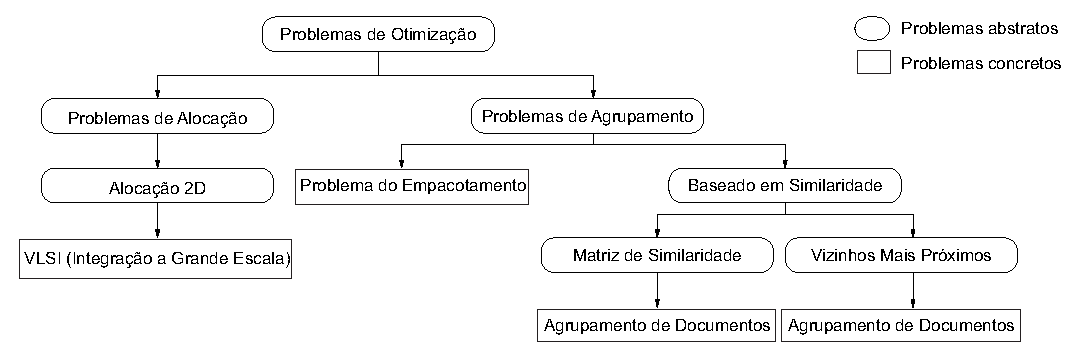
\includegraphics[width=1.0\textwidth]{problemasDeOtimizacao.eps}
%	\caption{Some Optimization Problems.\commentib{Falta apenas traduzir a imagem.} \label{fig:problemasDeOtimizacao}}
%	\end{figure*}
%	
%	An optimization problem can be defined as a finite set of variables, where the correct values for the variables specify the optimal solution. If the variables are of the set of real, the problem is called continuous, and if they can only have a finite set of distinct values, the problem is called combinatorial \protect\cite{francq2011optimization}.
%	
%	In order for the optimization problems to be solved, it is necessary to develop a method that solves them, which are the algorithms. An important category of problems are the NP-hard problems, where they can only be solved by certain algorithms that try to arrive at the optimal solution of that determined problem.
%	
%	When the optimal solution of an NP-hard problem is not guaranteed, this type of method is called a heuristic. A heuristic is an intuitive way of solving a particular problem, where the best possible solution is not guaranteed.
%	
%	Every optimization problem is basically characterized by having an objective function, which can be called cost function when it is desired to minimize it or utility function when it is desired to maximize it, and a set of constraints that delimit the space of viable solutions, or Be the region where the solutions are that can be accepted. The objective function contains a set of variables to which values must be assigned in a systematic way so as to walk through the search space and find the one that optimizes the result to be searched, in case a maximization problem finds the highest possible value while in a Minimize the value. In both cases the solution must satisfy the set of constraints imposed to be accepted. 


%	One can interpret the space of solutions as being a subset of Euclidean space \(\R^n\). Each variable is a dimension of space. For a function with two variables it is possible to form in a two-dimensional space and with the addition of a third dimension to the result of the function with \(x\) and \(y\) as input it is possible to observe the behaviour of the function as The \(x\) and the \(y\) of the function undergo variation. In Figure ~\ref{fig:sol} a two-dimensional graph is shown in which the variation of the function value causes changes in the gray scale. For larger values ??a darker gray is obtained and for smaller values ??a lighter gray is obtained. With this, one can observe the space of solutions in a panoramic way in the two-dimensional space and it is verified that as it approaches the center the function generates smaller values. In it it is also possible to notice that the x-shaped marks, which represent the solutions found, vary towards the local minimum that is in the middle of the search space. The heuristic used to search for the optimal solution in this case was to look for neighbouring solutions that minimized the cost of the function in the same way that a sphere that rolls over an inclined plane stabilizes when it reaches a valley that would be the local minimum Function. However, this heuristic is not always the most adequate, as will be seen later.
%
%\begin{figure}[H]
%	\centering
%	\includegraphics[width=0.5\textwidth]{sol.eps}
%	\caption{Walking through the space of solutions\label{fig:sol}}
%\end{figure}

%%%%%%%%%%%%%%%
\section{UAV Movement System}
\label{sec:uav}
%%%%%%%%%%%%%%%

% \subsection{UAV Movement System}

%In this section, we first investigate the UAV platform used (3DR IRIS+) in this study, describing the hardware characteristics and the control framework developed for intralogistics missions. 
The core hardware of the UAV IRIS+ is the Pixhawk and we can control it using a Python library \cite{dronekit}, which uses Micro Air Vehicle Link (MAVLink) protocol~\cite{meier2011pixhawk}. MAVLink is a protocol for communicating with small unmanned vehicle, which is designed as a header-only message marshalling library.

The IRIS+ UAV is integrated into a robot gripper to take and leave packages during missions (cf. Definition~\ref{def:mission}). We have connected a servo motor to the Pixhawk by one of the pulse width modulation (PWM) outputs. Figure~\ref{fig:hardArch} shows the system hardware architecture and the interconnections between each component module. In the hardware architecture shown in the Figure~\ref{fig:hardArch}, we can see the UAV hardware component connections where there is the Pixhawk (flight controller) and its connections between other components such as the compass, GPS, PWM outputs, battery and etc. Moreover, it shows the connection with a robot gripper using a PWM outputs as a signal control for the servo motor in the robot gripper. Finally, it shows the communication between a personal computer (PC) and the UAV via radio control (RC) signal.
%
\begin{figure}[H]
	\centering
	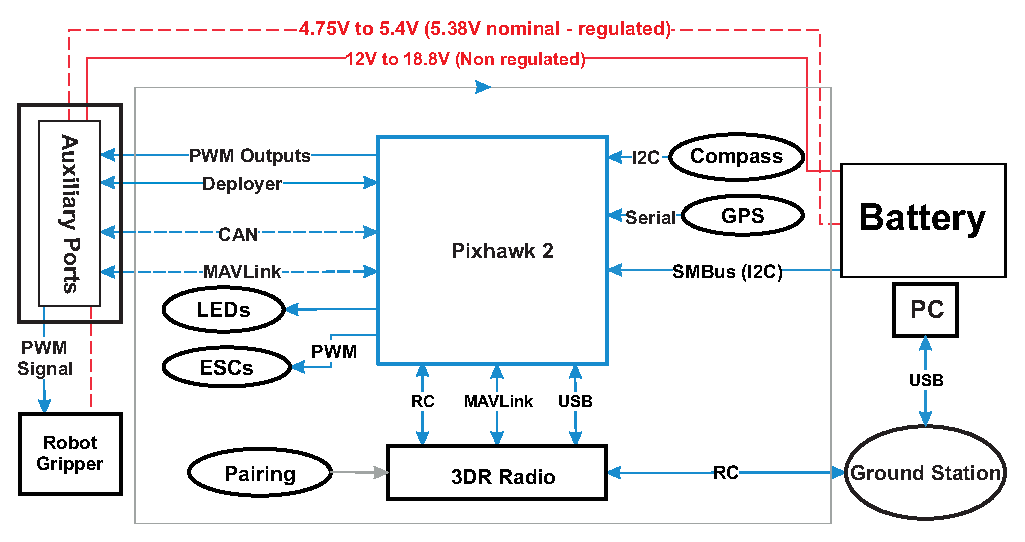
\includegraphics[width=\columnwidth]{arquiteturaIHW.eps}
	\caption{System Hardware Architecture.}
	\label{fig:hardArch}
\end{figure}

In the software architecture, the Mission Planner (cf. Definition~\ref{def:planejadorMissao}) reads the warehouse inputs and client order and produces a \texttt{.mission} file, which contains the list of mission commands needed for producing the required client order. This \texttt{.mission} file is used by a UAV Control Program to control the UAV and to produce the low-level movement commands using MAVLink protocol (cf. Definition~\ref{def:missioncommand}). Figure~\ref{fig:sysArch} shows the mission planning framework software components.


In order to control the UAV from a PC, we have used the dronekit API that translates MAVLink commands to a Python function. In the ground station, the PC is running the UAV Control Program that controls the UAV using a radio module connected to the PC via USB. We have created a bunch of functions in the control program for the most common UAV actions. The movement functions (cf. Definition~\ref{def:movFunc}) are described in Table~\ref{table:movfunc}.
%
%\begin{itemize}
%\item \texttt{TakeOff}: takeoff command of the UAV;
%\item \texttt{GoTo}: command to move the  UAV to a certain location;
%\item \texttt{TakePackage}: command to collect an input/product through a robot gripper;
%\item \texttt{LeavePackage}: command to leave an input or product from a robot gripper;
%\item \texttt{Wait}: command to make a UAV to hover (wait);
%\item \texttt{Land}: command to make a UAV to land.
%\end{itemize}

\begin{table}[]
\scriptsize
\centering
\begin{tabular}{|l|l|}
\hline
\multicolumn{1}{|c|}{\textbf{Command}} & \multicolumn{1}{c|}{\textbf{Description}}           \\ \hline
\texttt{TakeOff}                     & takes off the UAV                                   \\ \hline
\texttt{GoTo}                        & moves the UAV to a certain location                 \\ \hline
\texttt{TakePackage}                 & takes an input/product (gripper) \\ \hline
\texttt{LeavePackage}                & leaves an input/product (gripper)   \\ \hline
\texttt{Wait}                        & makes the UAV to hover (wait)                       \\ \hline
\texttt{Land}                        & lands the UAV                                       \\ \hline
\end{tabular}
\caption{Description of movement functions}
\label{table:movfunc}
\end{table}


\begin{figure}[H]
	\centering
	\includegraphics[width=\columnwidth]{sysArch.eps}
	\caption{System's Architecture.\label{fig:sysArch}}
\end{figure}


%\subsection{Mission Planning}
%\label{mission}


%%%%%%%%%%%%%%%
\section{Methodology of Time Cost Evaluation, UAV Use and Mission Planning}
\label{sec:method}
%%%%%%%%%%%%%%%

%\commentib{Modifique o t\'itulo (expanda). Metodologia de qu\^e?? Tente fazer algo parecido com o do trabalho.}

%In this section, we evaluate the algorithm mission cost and describe a case study to a UAV and contents about mission planning.

%%%%%%%%%%%%%%%%%%%%%%%%%%%%%%%%%%%%%
\subsection{Case Study: UAV Intralogistics Mission}
\label{sec:ec}
%%%%%%%%%%%%%%%%%%%%%%%%%%%%%%%%%%%%%

In order to model the mission planning problem as an optimization problem, the case study shown in Figure~\ref{fig:useCase} is used.
%
\begin{figure}[ht]
	\centering
	\includegraphics[width=0.85\columnwidth]{useCase.eps}
	\caption{Case Study Representation.\label{fig:useCase}}
\end{figure}
	
Figure~\ref{fig:useCase} shows that there are three types of inputs in the warehouse (\textit{i.e.}, A, B, and C) and two production lines that produce two different products (\textit{i.e.}, X and Y). Each production line produces only one type of product and has a characteristic production time (cf. Definition~\ref{def:tempoProducao}). Figure~\ref{fig:useCase} shows that to produce a product of type X, two inputs of type A and one input of type C are required, and to produce a product of type Y, two inputs of type B and one input of type C are required. The production time of a X product is $4 p.u.$ and the time of production of product Y is $6 p.u.$. A production unit ($1 p.u.$) is considered to be a \texttt{GoTo} command performed by the UAV.

The task to be performed is the production of the client order (cf. Definition~\ref{def:pedido}), where a given UAV collects supplies from the warehouse, takes that to the production line, and once the production of a certain product is finished, the UAV delivers it to the client.

%%%%%%%%%%%%%%%
\subsection{Modeling a UAV Intralogistics Mission as an Optimization Problem }
\label{ssec:modelo}
%%%%%%%%%%%%%%%

The purpose of this subsection is to make the mission planning problem into an optimization problem, creating a modeling for the problem; in order to find, afterwards, the shortest execution time of all tasks (minimization), based on the case study explained in Section~\ref{sec:ec}. The notation used is given below:

\begin{itemize}
\item $\mathcal{T} = \set{T_j \vert j\in \mathbb{N}^{*},j\leq N}$ is the set of $N$ tasks;
\item $\mathcal{M} = \set{m_i \vert i\in \mathbb{N}^{*},i\leq M}$ is the set of $M$ production lines (machines);
\item $\mathcal{P} = \set{p_j \vert j\in \mathbb{N}^{*},j\leq N}$ is the processing time of each $j$-th task;
\item $S = \set{s_i \vert s\in \mathbb{N}^{*},i\leq M}$  is the setup (production) time of each $i$-th production line;
%\item $R||C_{max}$ (Three-field notation\footnote{Notation $\alpha | \beta | \gamma$, where $\alpha$: processing environment, $\beta$: problem constraints and $\gamma$: optimization criterion.} used in the literature to represent a given task scheduling problem, in this case, minimizing the makespan \footnote{Makespan is the termination time of the most loaded processor.\label{nt:makespan}} in an unrelated parallel machine environment \cite{graham1979optimization}.
\end{itemize}

\paragraph{Decision variable}

The variable $x_{ij}$ is a binary decision variable that takes the value $1$ if the task $j$ is running on the machine $i$; and $0$ otherwise. The variable $C_ {mission}$ is the variable that we want to optimize.
%
\begin{equation}
\label{eq:decision}
\begin{split}
x_{ij}=\begin{cases}
    1,       & \quad \text{if the task } j \text{ is running in} \\
 &\text{ the machine (production line) }i\\
    0,  & \quad \text{otherwise}\\
  \end{cases}
\end{split}
\end{equation}

\paragraph{Objective function}

The objective function is the total mission cost $C_{mission}$ (total process execution time) that can be modeled as follows.
%
\begin{equation}
\label{eq:objfunction}
C_{mission}=\sum_{i=1}^{M}{\sum_{j=1}^{N}{
 (p_j+s_i)x_{ij}}},
\end{equation}

Eq.~\eqref{eq:objfunction} represents the sum of the duration time $p_j$ of each travel from one place to another in the case study explained in Section~\ref{sec:ec}, considering the production time (cf. Definition~\ref{def:tempoProducao}) $s_j$ in each production line.

%\begin{equation}
%\label{eq:cmax}
%C_{max} = \sum_{i=1}^{M}{\sum_{j=1}^{N}{
% (p_j+s_j)x_{ij}}}
%\end{equation}


\paragraph{Constraints}

\begin{itemize}
\item Each task must be executed/processed in a unique machine:

\begin{equation}
\label{eq:unicity}
\sum_{i=1}^{M}{\sum_{j=1}^{N}{x_{ij}}}=1
\end{equation}

\item Execution time of each machine:

\begin{equation}
\label{eq:execTime}
C_{mission}\leq C_{max}
\end{equation}

Eq.~\eqref{eq:execTime} indicates that the mission cost is always less or equal than a maximum cost denoted by $C_{max}$, obtained empirically.
\end{itemize}

% For a better understanding what the summation means, let's suppose that there are two production lines and tree products to be produced (tasks), therefore, $x_{00}+x_{10}+x_{20}=1$, $x_{01}+x_{11}+x_{21}=1$ and $x_{02}+x_{12}+x_{22}=1$, so, it can be verified that those restrictions are set, there will be only one task running in a machine.

\paragraph{Resulting optimization problem}

The resulting optimization problem consists in minimizing $C_{max}$ w.r.t. the decision variable \eqref{eq:decision} constrained to the condition in Equations \eqref{eq:unicity} and \eqref{eq:execTime}. Thus, the optimization problem is represented as follows:
%
\begin{equation}
	\label{eq:optproblem}
	\begin{array}{ccc}
		\min & C_{mission},  \\
  \\
		\textrm{ s.t. } & \sum_{i=1}^{M}{\sum_{j=1}^{N}{x_{ij}}}=1, \\
		& C_{mission}\leq C_{max}
 \\
	\end{array}
\end{equation}	
%
%{\color{red}
%Model:
%
%\begin{enumerate}
%\item \textbf{Choosing the constraints:}
%
%
%
%\begin{equation}
%C_{max}=makespan \text{ (duration of a mission)}
%\end{equation}
%\item \textbf{Elaboration of the objective function:}
%The objective function is the variable $C_{max}$ (total process execution time) that needs to be minimized.
%\begin{equation}
%\text{Minimize } C_{max}
%\end{equation}
%$C_{max}$ is the variable that need to be minimized (optimized).
%\item \textbf{Restrictions:}
%
%\begin{itemize}
%\item \textbf{Each task must be executed/processed in an unique machine (production line)}
%
%\begin{equation}
%\sum_{\substack{
%   i \in M\\
%   \forall j \in J
%  }} 
% x_{ij}=1
%\end{equation}
%
%For a better understanding what the summation means, let's suppose that there are two production lines and tree products to be produced (tasks), therefore, $x_{00}+x_{10}+x_{20}=1$, $x_{01}+x_{11}+x_{21}=1$ and $x_{02}+x_{12}+x_{22}=1$, so, it can be verified that those restrictions are set, there will be only one task running in a machine.
%
%\item \textbf{Time execution of the tasks in each machine}
%
%
%
%For a better understanding what the summation means, let's suppose that there are two machines and two tasks, and the time of processing and setup of each task are $p_0=100,~ p_1=100$ and $s_0=12,~ s_1=18$ respectively. Therefore, the production time of the product $0$ in the production line $0$ is $p_0 + s_0$ and so on. 
%\end{itemize}
%\item \textbf{Completeness and non-negativity:}
%
%\begin{equation}
%\begin{split}
% x_{ij} \in \{0,1\}~\forall i=1,2,...,M\text{ and }\\
% \forall j=0(dummy), 1,2,3,...,N
%\end{split}
%\end{equation}
%
%\item \textbf{Full model:}
%\begin{align*}
%\begin{split}
%\text{Minimize~~~}  & C_{max} \\
%    \text{Subject to~~~}  &\sum_{\substack{
%   i \in M\\
%   \forall j \in J
%  }} 
%  x_{ij}=1 \\
%    & \sum_{\substack{
%   j \in J\\
%   \forall i \in M
%  }} 
% (p_j+s_j)x_{ij}\leq C_{max} \\
% 	& x_{ij} \in \{0,1\}~\forall i=1,2,...,M ~e~
% 	\forall \\
% &j=0(dummy), 1,2,3,...,N
%\end{split}
%\end{align*}
%
%\end{enumerate}
%}
%%%%%%%%%%%%%%%
\subsection{Planner Evaluation Methodology}
\label{ssec:evaluationmethod}
%%%%%%%%%%%%%%%

The main contribution of this study is a methodology to evaluate UAV mission planner algorithms and to find minimum cost planner. For this purpose, a generalized evaluation metrics is developed. The objective (cost) function modeled in Section~\ref{ssec:modelo} is related to the total time spent for the mission execution. Our evaluation metrics compares the cost of a planner algorithm with the best cost computed by the CPLEX solver~\cite{cplex2003ilog}. This work proposed a novel metrics called Mission Planner Cost Index ($MPCI$).

Firstly, the optimal cost of the problem is obtained by means of the CPLEX solver, which returns the optimum value (minimum mission execution time). The model proposed in Section~\ref{ssec:modelo} is implemented using the CPLEX solver library available for C++. 

The cost of each planner strategy (Algorithms~\ref{alg:planA} and~\ref{alg:planB}) $c_X$ is obtained by counting the number of \texttt{GoTo} commands which represents a process (task).

Finally, the evaluation of each mission planner is computed w.r.t. the optimal cost, therefore, the $MPCI_{X}$ of a planner $X$ is computed as follows:
%
\begin{equation}
\label{eq:MPCI}
	MPCI_X=\frac{c_o}{c_X},
\end{equation}

\noindent where $c_o$ is the optimal cost obtained by a C++ program that converts a given instance to a file in a format known by CPLEX, such as the LP format, \textit{i.e.} the developed algorithm generates the model to be solved by CPLEX with the help of the mathematical programming tool UFFLP. \textbf{$c_X$} is the cost of the solution generated by planner $X$, and $0 \leq MPCI_X \leq 1$. Note that as close to $1$ the $MPCI_X$ is, the solution cost becomes smaller.

\subsection{Mission Planners}

In this study, we considered that mission planner is a software that generates a production mission (cf. Definition~\ref{def:prodMission}) given the warehouse and customer order. This program generates a \texttt{.mission} extension file containing a set of mission commands (cf. Definition~\ref{def:missioncommand}), as described in Section~\ref{sec:uav}. Two examples of planners are presented in this work and are employed to demonstrate the cost evaluation methodology.

\subsubsection{Planner 1}

In Algorithm~\ref{alg:planA}, we show a strategy to solve the mission planning problem and we denoted it as Planner 1. In this particular algorithm, the production of X products has a higher priority over Y, {\it i.e.}, the inputs are firstly allocated to production of X orders, and the production of Y products begins if there is no other X to be produced. The general steps of planner 1 are described in Algorithm~\ref{alg:planA}.
%
\begin{algorithm}[ht]
\scriptsize
\KwIn{warehouse}
\KwIn{order}
\KwOut{mission file \textit{.mission}}
\Begin{
check the order\;
\Repeat{production of all X elements finish}{
go to the warehouse\;
\Repeat{bring 2 A elements}{
	get input A\;
	bring to the production line X\;
}
go to the warehouse\;
get the input C\;
bring to the production line X\;
wait X to be produced\;
bring X to the client\;
}
\Repeat{production of all Y elements finish}{
go to the warehouse\;
\Repeat{bring 2 B elements}{
	get input B\;
	bring to the production line Y\;
}
go to the warehouse\;
get the input C\;
bring to the production line Y\;
wait Y to be produced\;
bring Y to the client\;
}
}
\captionsetup{list=no}
\caption{Planner 1}\label{alg:planA}
\end{algorithm}

\subsubsection{Planner 2}

The strategy for Planner 2 is a bit more complex than Planner 1. In the Planner 2 strategy, the UAV starts to bring all the necessary inputs to make the first X product, taking all the A, B and C inputs, respectively, to the production line X. After bring all the necessary inputs to produce the first X product, the production line X starts to produce the X product and while the production line X is producing, the UAV goes to the warehouse to get the necessary inputs to produce the next product (either Planner 1 and Planner 2 produce firstly the X products e then all the Y products). However, when the X product finishes producing, the UAV knows the instant and goes to the production line to get the X product to bring to the client place; and after that, the UAV goes back to bring the rest of the inputs. The UAV keeps work in the same way until it brings all the products to the client place. Differently to the Planner 1, the Planner 2 does not wait the production in the production line. The UAV works as a scheduler and executes the mission faster than Planner 1 strategy, because it does not enter in a busy wait state. The general steps of planner 2 are shown in the Algorithm~\ref{alg:planB}.
%
\begin{algorithm}[ht]
\scriptsize
\KwIn{warehouse}
\KwIn{order}
\KwOut{mission file \textit{.mission}}
\Begin{
initialize $t_x$\;
initialize $t_y$\;
check the order\;
\Repeat{production of all X elements finish}{
\uIf{the counter of that X is not $t_X$}{
go to the warehouse\;
\Repeat{until bring 2 A elements}{
	get the input A\;
	bring to the production line X\;
}
go to the warehouse\;
get the input C\;
bring to the production line X\;
start the counter of this X (production time)\;
keep producing\;
}
\Else{go back to the production line X\;
		bring X to the client\;
		go back to producing\;}
}
\Repeat{production of all Y elements finish}{
\uIf{the counter of that Y is not $t_Y$}{
go to the warehouse\;
\Repeat{until bring 2 B elements}{
	get the input B\;
	bring to the production line Y\;
}
go to the warehouse\;
get the input C\;
bring to the production line Y\;
start the counter of this Y (production time)\;
keep producing\;
}
\Else{go back to the production line Y\;
		bring Y to the client\;
		go back to producing\;}
}
}
\captionsetup{list=no}
\caption{Planner 2}\label{alg:planB}
\end{algorithm}

Where $t_X$ and $t_Y$ are the production time (cf. Definition~\ref{def:tempoProducao}) of the production lines X and Y, respectively.


%%%%%%%%%%%%%%%%%%%%%%%%%%%%%%%%%%%%%
\section{Experimental Evaluation}
\label{sec:results}
%%%%%%%%%%%%%%%%%%%%%%%%%%%%%%%%%%%%%

This section describes the experimental results obtained in this project, as well as the cost evaluation of two techniques used, which are compared to the optimum cost implemented with the CPLEX solver.

%%%%%%%%%%%%%%%%%%%%%%%%%%%%%%%%%%%%%
\subsection{Experimental Environment and Objectives}
\label{ssec:expobjandenv}
%%%%%%%%%%%%%%%%%%%%%%%%%%%%%%%%%%%%% 
In order to verify the efficiency of the metrics shown in Section~\ref{sec:method}, our experimental evaluation aims to answer the following research questions:
\begin{enumerate}

\item[RQ1] Does the framework for mission planning, command and control for intralogistics mission using a UAV produce the expected results?

\item[RQ2] Is the metrics of mission evaluation efficient?

\end{enumerate}

The mission planning algorithms were executed in a computer running Linux Mint OS, core i7 processor and 8 GB of RAM. In order to control the UAV, we run the control program, which uses the dronekit API as an interface between a high level program language (Python) and the protocol that the UAV understands (MAVLink), in the same computer where there is a radio module connected via USB communicating with the UAV radio module.


\subsection{Cost Evaluation}
\label{ssec:acusto}

The results of each mission planner is compared to the optimal solution obtained with the branch-and-cut algorithm of the IBM/ILOG CPLEX 12.4 tool developed in C++ \cite{cplex2003ilog}. In order to obtain better results to perform the comparison, it was considered only the time in which the UAV takes to finish the production of a product.

\begin{table}[H]
\centering
\footnotesize

\begin{tabular}{c|c|c|c|}
\cline{2-4}
                                        & \textbf{Planner 1} & \textbf{Planner 2} & \textbf{CPLEX} \\ \hline
\multicolumn{1}{|c|}{\textbf{Time (s)}} & 420                & 404                & 134            \\ \hline
\end{tabular}
\caption{Planners and optimal (CPLEX) times}
\label{fig:comp}
\end{table}

The Table~\ref{fig:comp} shows the mission execution times obtained using the planner algorithms 1 and 2, and the minimum value provided by CPLEX. Using the metrics shown in the section~\ref{sec:method}, then:

\begin{equation}
\small
MPCI_1=\frac{134}{420}=0.319
\label{eq1}
\end{equation}


\begin{equation}
\small
MPCI_2=\frac{134}{408}=0.328
\label{eq2}
\end{equation}

The MPCI indicates (cf. Eqs.~\eqref{alg:planA} and \eqref{alg:planB}) that planner 2 performs the mission more quickly and has a lower cost than planner 1.

\subsection{Practical Results}

In order to verify the practical results, as well as a cost comparison between the different approaches of mission planners developed in this work, the flight time measurement was performed using the two mission planning algorithms developed, using the case study shown in \ref{sec:ec}.

The experiments were performed in both, simulator and real UAV system. The simulations are performed with DroneKit-SITL~\cite{dronekit}, that is an resource of Dronekit Pythn API that allows to simulate the behavior and movement of a plane, a copter, or a rover, without the hardware, {\it i.e.} a real UAV.  Additional experiments are performed with the real UAV system (3DR IRIS+). Figure~\ref{fig:maps} shows the map of experimental environment (Faculty of Physical Education and Physiotherapy of Federal University of Amazonas).

		\begin{figure}[H]
	\centering
	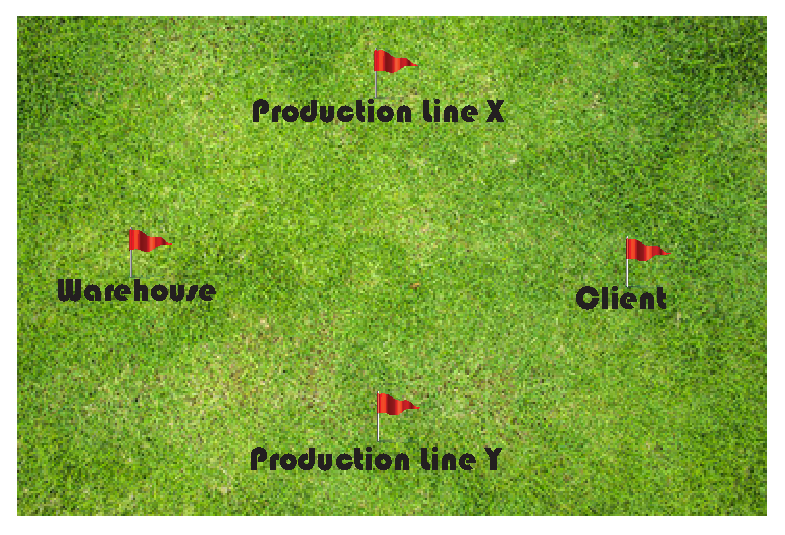
\includegraphics[width=0.7\columnwidth]{map.eps}
	\caption{Warehouse, Production Line X, Production Line Y and Costumer in the Map.\label{fig:maps}}
	\end{figure}
%           
%Below, we can verify the two mission files generated by the two strategies developed in this work:

%\begin{figure}[H]
%\centering
%\begin{subfigure}{.5\textwidth}
%  \centering
%  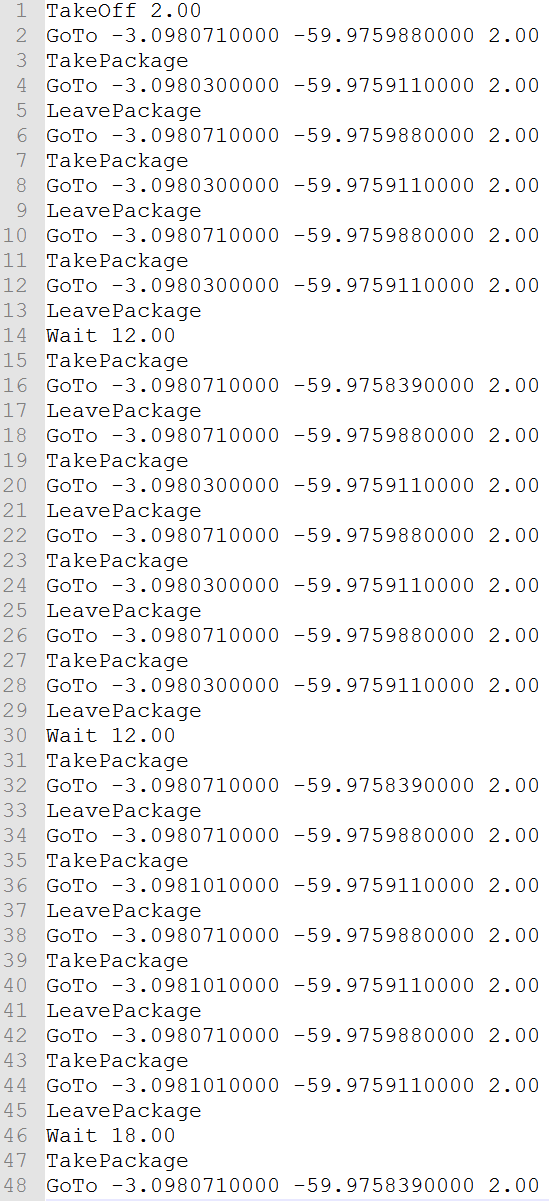
\includegraphics[width=.6\linewidth]{planAArq.PNG}
%  \caption{Planejador A.}
%  \label{fig:planAArq}
%\end{subfigure}%
%\begin{subfigure}{.5\textwidth}
%  \centering
%  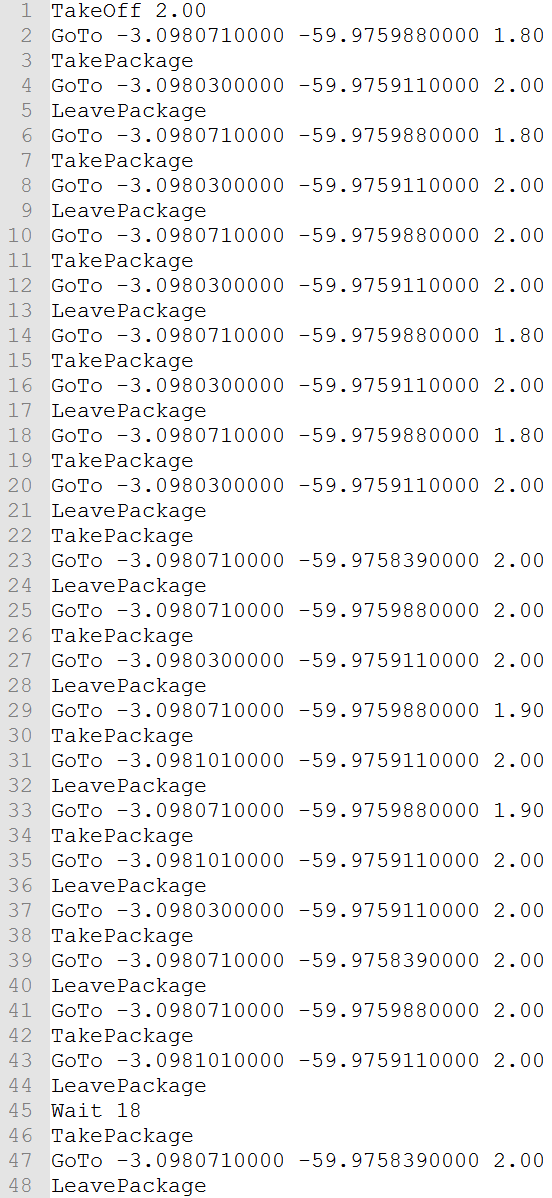
\includegraphics[width=.6\linewidth]{planBArq.PNG}
%  \caption{Planejador B.}
%  \label{fig:planBArq}
%\end{subfigure}
%\caption{Arquivos de Missão.}
%\label{fig:planArq}
%\end{figure}

%The two mission files shown above, have exactly the same instances, that is, they have the same resources and have to perform the same mission that is to produce two products of type X and one of type Y. However, they execute the mission of Different way and have different performances. As discussed in Section~\ref{sec:acusto}, planner 2 has more \texttt{GoTo} commands than planner 1 (see Figure~\ref{fig:planArq}).

Table~\ref{table:plannersReal} presents the performance (total flight time) of both planners algorithms for simulations and tests with the (real) 3DR Iris+ UAV.

	\begin{table}[H]
\footnotesize
\centering
\begin{tabular}{|c|c|c|c|c|}
\hline
\multirow{3}{*}{\textbf{\begin{tabular}[c]{@{}c@{}}Test\\ \#\end{tabular}}} & \multicolumn{4}{c|}{\textbf{Flight Time of Planners}}                                 \\ \cline{2-5} 
                                                                            & \multicolumn{2}{c|}{\textbf{Simulator}}   & \multicolumn{2}{c|}{\textbf{3DR Iris+}}   \\ \cline{2-5} 
                                                                            & \textit{\textbf{1}} & \textit{\textbf{2}} & \textit{\textbf{1}} & \textit{\textbf{2}} \\ \hline
\textit{\textbf{1}}                                                         & 460.41              & 436.08              & 455.12              & 441.72              \\ \hline
\textit{\textbf{2}}                                                         & 460.69              & 436.89              & 456.93              & 440.18              \\ \hline
\textit{\textbf{3}}                                                         & 460.08              & 441.68              & 457.19              & 447.51              \\ \hline
\textit{\textbf{4}}                                                         & 460.72              & 441.03              & 460.25              & 438.19              \\ \hline
\textit{\textbf{5}}                                                         & 460.23              & 451.87              & 459.47              & 445.85              \\ \hline
\end{tabular}
\caption{Mission Planners Flight Times.\label{table:plannersReal}}
\end{table}



Table~\ref{table:plannersReal} indicates that the mission time of planner 2 is lower than the time of planner 1 in all five tests with simulator and 3DR Iris+, ensuring the results of the evaluation methodology.
%Figure~\ref{fig:GraPlannersSimulado} shows a bar graph of the simulation flight times of both planners in the five tests.
%
%\begin{figure}[H]
%	\centering
%	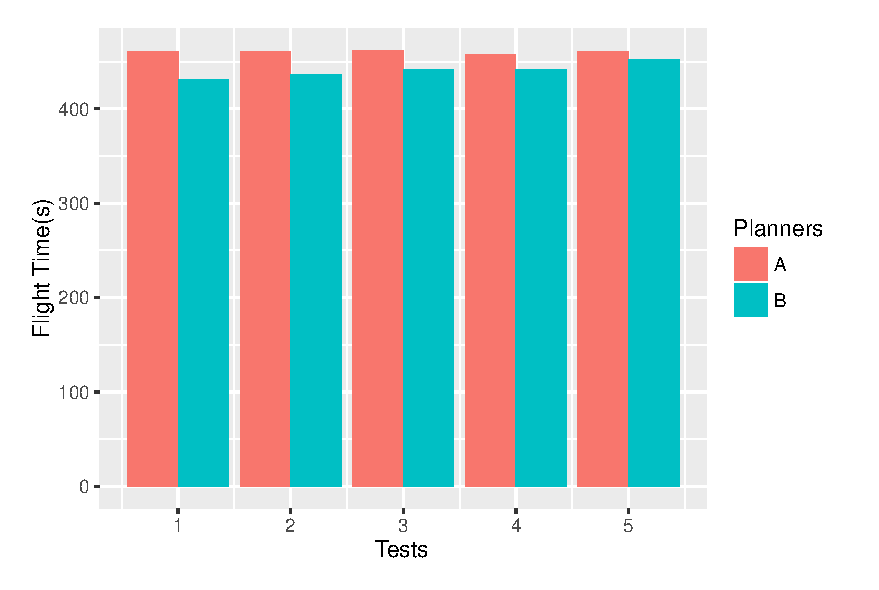
\includegraphics[width=0.7\columnwidth]{GraPlannersSimulado.eps}
%	\caption{Flight Time Graph of Mission Planners Relative to 5 Tests in Simulator.\label{fig:GraPlannersSimulado}}
%	\end{figure}
	

	
%
%Figure~\ref{fig:GraPlannersReal} shows a bar graph of the flight times of both planners in the five tests with IRIS+.
%
%\begin{figure}[H]
%	\centering
%	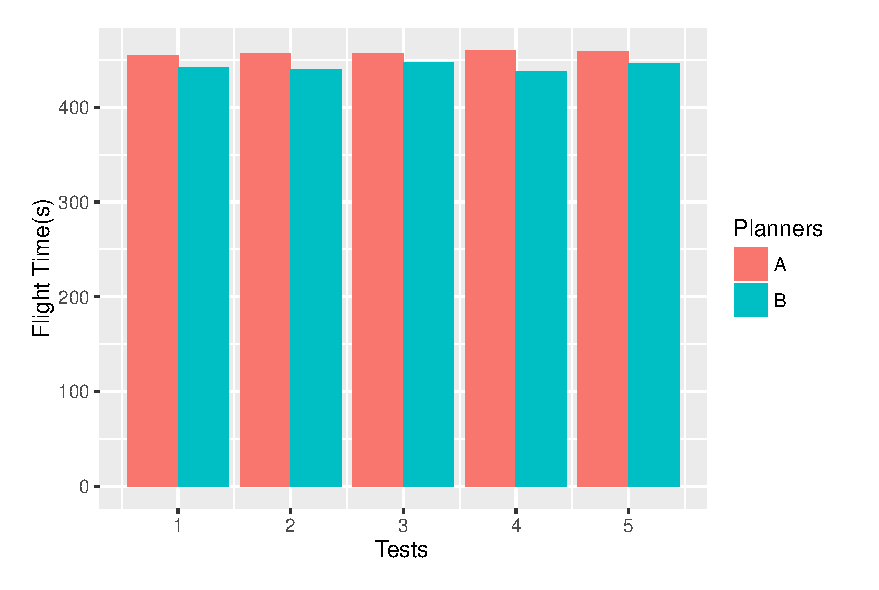
\includegraphics[width=0.7\columnwidth]{GraPlannersReal.eps}
%	\caption{Flight Time Graph of Mission Planners Relative to 5 Tests in a Real Environment.\label{fig:GraPlannersReal}}
%	\end{figure}
	
	The aforementioned results confirmed the prediction provided by the planner evaluation methodology, and the planner 2 is faster than planner 1 in all the tests with simulations and IRIS+ tests.
	
\subsection{Threats to Validity}
\label{sec:ameacas}

In order to compile the experiments, we have assembled a favourable environment to apply our evaluation metrics. In this way, we considered the use case in Section~\ref{sec:method}.

However, in case we change the scenario where the number of UAVs increases, our algorithms will not work as expected because we did not adapted the algorithms for cooperative work and consequently our metrics will not work as expected. Further works may be implemented to make the metrics works in a cooperative work environment where the number of UAVs is greater than two.

%\textcolor{red}{Thiago, nao ficou claro pra mim os objetivos dos experimentos... poderias escrever claramente quais seriam as research questions que devemos responder nos experimentos? Alem disso, precisas descrever uma secao sobre ameacas da validade dos resultados... como exemplo, olhe este artigo: https://arxiv.org/pdf/1610.04761.pdf}

% An example of a floating figure using the graphicx package.
% Note that \label must occur AFTER (or within) \caption.
% For figures, \caption should occur after the \includegraphics.
% Note that IEEEtran v1.7 and later has special internal code that
% is designed to preserve the operation of \label within \caption
% even when the captionsoff option is in effect. However, because
% of issues like this, it may be the safest practice to put all your
% \label just after \caption rather than within \caption{}.
%
% Reminder: the "draftcls" or "draftclsnofoot", not "draft", class
% option should be used if it is desired that the figures are to be
% displayed while in draft mode.
%
%\begin{figure}[!t]
%\centering
%\includegraphics[width=2.5in]{myfigure}
% where an .eps filename suffix will be assumed under latex, 
% and a .pdf suffix will be assumed for pdflatex; or what has been declared
% via \DeclareGraphicsExtensions.
%\caption{Simulation results for the network.}
%\label{fig_sim}
%\end{figure}

% Note that the IEEE typically puts floats only at the top, even when this
% results in a large percentage of a column being occupied by floats.


% An example of a double column floating figure using two subfigures.
% (The subfig.sty package must be loaded for this to work.)
% The subfigure \label commands are set within each subfloat command,
% and the \label for the overall figure must come after \caption.
% \hfil is used as a separator to get equal spacing.
% Watch out that the combined width of all the subfigures on a 
% line do not exceed the text width or a line break will occur.
%
%\begin{figure*}[!t]
%\centering
%\subfloat[Case I]{\includegraphics[width=2.5in]{box}%
%\label{fig_first_case}}
%\hfil
%\subfloat[Case II]{\includegraphics[width=2.5in]{box}%
%\label{fig_second_case}}
%\caption{Simulation results for the network.}
%\label{fig_sim}
%\end{figure*}
%
% Note that often IEEE papers with subfigures do not employ subfigure
% captions (using the optional argument to \subfloat[]), but instead will
% reference/describe all of them (a), (b), etc., within the main caption.
% Be aware that for subfig.sty to generate the (a), (b), etc., subfigure
% labels, the optional argument to \subfloat must be present. If a
% subcaption is not desired, just leave its contents blank,
% e.g., \subfloat[].


% An example of a floating table. Note that, for IEEE style tables, the
% \caption command should come BEFORE the table and, given that table
% captions serve much like titles, are usually capitalized except for words
% such as a, an, and, as, at, but, by, for, in, nor, of, on, or, the, to
% and up, which are usually not capitalized unless they are the first or
% last word of the caption. Table text will default to \footnotesize as
% the IEEE normally uses this smaller font for tables.
% The \label must come after \caption as always.
%
%\begin{table}[!t]
%% increase table row spacing, adjust to taste
%\renewcommand{\arraystretch}{1.3}
% if using array.sty, it might be a good idea to tweak the value of
% \extrarowheight as needed to properly center the text within the cells
%\caption{An Example of a Table}
%\label{table_example}
%\centering
%% Some packages, such as MDW tools, offer better commands for making tables
%% than the plain LaTeX2e tabular which is used here.
%\begin{tabular}{|c||c|}
%\hline
%One & Two\\
%\hline
%Three & Four\\
%\hline
%\end{tabular}
%\end{table}


% Note that the IEEE does not put floats in the very first column
% - or typically anywhere on the first page for that matter. Also,
% in-text middle ("here") positioning is typically not used, but it
% is allowed and encouraged for Computer Society conferences (but
% not Computer Society journals). Most IEEE journals/conferences use
% top floats exclusively. 
% Note that, LaTeX2e, unlike IEEE journals/conferences, places
% footnotes above bottom floats. This can be corrected via the
% \fnbelowfloat command of the stfloats package.




\section{Conclusion}
\label{sec:conclusao}
%---------------------------------

We have presented an evaluation methodology for UAV mission planner in an industrial production scenario, as described in Section~\ref{sec:method}. We have used a evaluation methodology to perform two different algorithms to verify the performance of them. Our approach uses an optimizer tool to generate an optimal cost for a mission (w.r.t. flight time) and compares to different algorithm strategies using the index defined in Eq.~\ref{eq:MPCI}.
 
In addition, we have developed a framework for mission planning, command and control for intralogistics mission using a commercial UAV. We used an UAV to solve intralogistics problems using the dronekit API to control and command adopting a high-level programming language.

Summary, our experiments to test the evaluation methodology for mission planner were done successfully as expected in simulated environment as well as in a real environment using a real UAV, and consequently, the methodology is able to evaluate mission planner algorithms for intralogistics problems. Moreover, the framework can solve the necessity of control and command a commercial UAV. Thus, our work is a new tool to verify a specific problem of intralogistics.

Future work includes the use of computational vision for the recognition of inputs, and improvements of the optimization problem modeling for better results in cost evaluation. Supplementary, we will make experiments in a cooperative work environment where the number of UAVs is greater than two. In order to improve our results, we will develop more planner strategies such as an algorithm that produces different types of products simultaneously.




% conference papers do not normally have an appendix


% use section* for acknowledgment
\section*{Acknowledgment}


The authors would like to thank...





% trigger a \newpage just before the given reference
% number - used to balance the columns on the last page
% adjust value as needed - may need to be readjusted if
% the document is modified later
%\IEEEtriggeratref{8}
% The "triggered" command can be changed if desired:
%\IEEEtriggercmd{\enlargethispage{-5in}}

% references section

% can use a bibliography generated by BibTeX as a .bbl file
% BibTeX documentation can be easily obtained at:
% http://mirror.ctan.org/biblio/bibtex/contrib/doc/
% The IEEEtran BibTeX style support page is at:
% http://www.michaelshell.org/tex/ieeetran/bibtex/
%\bibliographystyle{IEEEtran}
% argument is your BibTeX string definitions and bibliography database(s)
%\bibliography{IEEEabrv,../bib/paper}
%
% <OR> manually copy in the resultant .bbl file
% set second argument of \begin to the number of references
% (used to reserve space for the reference number labels box)

%\begin{thebibliography}{1}

%\bibitem{IEEEhowto:kopka}
%H.~Kopka and P.~W. Daly, \emph{A Guide to \LaTeX}, 3rd~ed.\hskip 1em plus
%  0.5em minus 0.4em\relax Harlow, England: Addison-Wesley, 1999.
  

%\bibliography{exemplo}

%\end{thebibliography}

\bibliographystyle{IEEEtran}
\bibliography{IEEEabrv,exemplo}


% that's all folks
\end{document}


